\section{State of the Art and Related Work}
\begin{frame}{State of the Art}{Before our Paper}
    \begin{itemize}
        \item You saw how to count \textsc{xor}s
        \item This count is split in the \enquote{overhead} and the \textsc{xor}s needed for the field multiplication
        \item Thus for \textsc{Aes} we get $56+8\cdot3\cdot4 = 56+96 = 152$
        \item Finding a good matrix reduces now to find the cheapest elements for field multiplication
        \item There is a lot of work followng this line~\cite{FSE:SKOP15,FSE:LiuSim16,FSE:LiWan16,C:BeiKraLea16,ToSC:SarSye16,EPRINT:JeaPeySim17,ACISP:SarSye17,EPRINT:ZhoWanSun17,ToSC:LiWan17,AFC:SarSim16}
    \end{itemize}
\end{frame}

\begin{frame}{State of the Art}{Best known Results}
    \centering
    \begin{tabular}{lrr}
        \toprule
        \multicolumn{3}{c}{$4 \times 4$ matrices over $\mathrm{GL}(8,\mathbb{F}_2)$}                                                  \\
        \midrule
        Matrix                               & Naive & Literature \\
        \midrule
        \textsc{Aes} (Circulant)             &  152  & \textbf{7+96}   \\ \rowcolor{gray!10}
        \midrule
        \cite{FSE:SKOP15} (Subfield)         &  136  &    40+96   \\
        \cite{FSE:LiuSim16}  (Circulant)     &  128  &    32+96   \\ \rowcolor{gray!10}
        \cite{FSE:LiWan16}                   &  106  &    10+96   \\
        \cite{C:BeiKraLea16} (Circulant)     &  136  &    24+96   \\ \rowcolor{gray!10}
        \cite{ToSC:SarSye16} (Toeplitz)      &  123  &    27+96   \\
        \cite{EPRINT:JeaPeySim17} (Subfield) &  122  &    20+96   \\
        \bottomrule
    \end{tabular}
\end{frame}

\begin{frame}{Related Work I}{}
    \begin{columns}
        \begin{column}{0.75\textwidth}
            \centering
            
\includegraphics[width=\textwidth]{data/paar}
        \end{column}
        \begin{column}{0.2\textwidth}
            \centering
            \visible<2->{%
            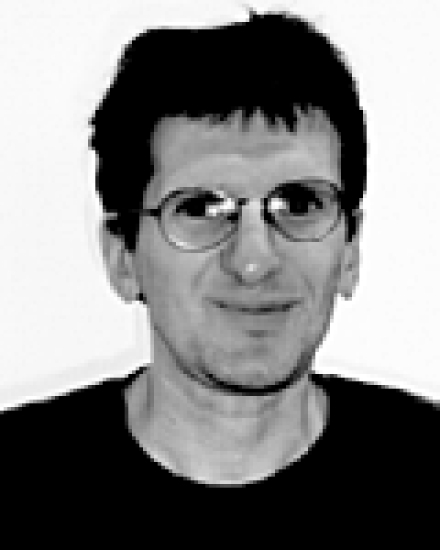
\includegraphics[width=\textwidth]{data/paar_ieeexplore}
            }
        \end{column}
    \end{columns}
\end{frame}

\begin{frame}{Related Work II}{}
    \begin{columns}
        \begin{column}{0.75\textwidth}
            \centering
            
\includegraphics[width=\textwidth]{data/joc}
        \end{column}
    \end{columns}
\end{frame}

\begin{frame}{State of the Art}{Best known Results (After our Paper)}
    \centering
    \begin{tabular}{lrrrrr}
        \toprule
        \multicolumn{6}{c}{$4 \times 4$ matrices over $\mathrm{GL}(8,\mathbb{F}_2)$}                                                  \\
        \midrule
                                             &       &            & \multicolumn{3}{c}{\visible<2->{Our Results~\cite{ToSC:KLSW17}}} \\
        Matrix                               & Naive & Literature & \visible<2->{\textsc{Paar1}} & \visible<2->{\textsc{Paar2}} & \visible<2->{\textsc{BP} }\\
        \midrule
        \textsc{Aes} (Circulant)             &  152  & \textbf{7+96} &   \visible<2->{108}       & \visible<2->{    108      }  & \visible<2->{     97     }\\ \rowcolor{gray!10}
        \midrule
        \cite{FSE:SKOP15} (Subfield)         &  136  &    40+96   &      \visible<2->{100}       & \visible<2->{     98      }  & \visible<2->{    100     }\\
        \cite{FSE:LiuSim16}  (Circulant)     &  128  &    32+96   &      \visible<2->{116}       & \visible<2->{    116      }  & \visible<2->{    112     }\\ \rowcolor{gray!10}
        \cite{FSE:LiWan16}                   &  106  &    10+96   &      \visible<2->{102}       & \visible<2->{    102      }  & \visible<2->{    102     }\\
        \cite{C:BeiKraLea16} (Circulant)     &  136  &    24+96   &      \visible<2->{116}       & \visible<2->{    112      }  & \visible<2->{    110     }\\ \rowcolor{gray!10}
        \cite{ToSC:SarSye16} (Toeplitz)      &  123  &    27+96   &      \visible<2->{110}       & \visible<2->{    108      }  & \visible<2->{    107     }\\
        \cite{EPRINT:JeaPeySim17} (Subfield) &  122  &    20+96   &      \visible<2->{ 96}       & \visible<2->{     95      }  & \visible<2->{ \textbf{86}}\\
        \bottomrule
    \end{tabular}
\end{frame}

\begin{frame}{State of the Art}{Finding better matrices?}
    \centering
    \begin{tabular}{lrlr}
        \toprule
        Type                                                    & \multicolumn{2}{c}{Previously Best Known} &  XOR count \\
        \midrule
        ${\mathrm{GL}(4, \mathbb{F}_2)}^{4 \times 4}$           &  $58$ & \cite{ToSC:SarSye16,EPRINT:JeaPeySim17} &  36  \\ \rowcolor{gray!10}
        ${\mathrm{GL}(8, \mathbb{F}_2)}^{4 \times 4}$           & $106$ & \cite{FSE:LiWan16}                &        72  \\
        $\parens{\mathbb{F}_2[x]/\mathtt{0x 13}}^{8 \times 8}$  & $392$ & \cite{FSE:SKOP15}                 &       196  \\ \rowcolor{gray!10}
        ${\mathrm{GL}(8, \mathbb{F}_2)}^{8 \times 8}$           & $640$ & \cite{FSE:LiuSim16}               &       392  \\
        \midrule
        $\parens{\mathbb{F}_2[x]/\mathtt{0x 13}}^{4 \times 4}$* &  $63$ & \cite{EPRINT:JeaPeySim17}         &        42  \\ \rowcolor{gray!10}
        ${\mathrm{GL}(8, \mathbb{F}_2)}^{4 \times 4}$           & $126$ & \cite{EPRINT:JeaPeySim17}         &        84  \\
        $\parens{\mathbb{F}_2[x]/\mathtt{0x 13}}^{8 \times 8}$  & $424$ & \cite{FSE:SKOP15}                 &       212  \\ \rowcolor{gray!10}
        ${\mathrm{GL}(8, \mathbb{F}_2)}^{8 \times 8}$           & $663$ & \cite{EPRINT:JeaPeySim17}         &       424  \\
        \bottomrule
    \end{tabular}
\end{frame}
